%CPET and Outcomes

\chapter{An investigation into the role of preoperative cardiopulmonary exercise testing in predicting adverse postoperative events after major pancreatic surgery.}
 
\label{ch_cpet_outcomes}
 
\lhead{Chapter \ref{ch_cpet_outcomes}. \emph{CPET and Postoperative Outcomes}} % This is for the header on each page - perhaps a shortened title
\clearpage
%----------------------------------------------------------------------------------------
 
\section{Introduction}
Pancreatic cancer is the tenth most common cancer in the UK but the fifth most common cause of cancer death with only 16-17\% surviving beyond the first year and 3\% surviving beyond 5 years. \parencite{cancerresearchuk_cancer_2014} The majority of patients (80-85\%) with pancreatic cancer present with inoperable disease.\parencite{cancerresearchuk_cancer_2014, sener_pancreatic_1999} In patients with resectable disease, surgery \parencite{sener_pancreatic_1999, sohn_resected_2000, geer_prognostic_1993} followed by adjuvant chemotherapy\parencite{neoptolemos_randomized_2004,neoptolemos_adjuvant_2009} remains the primary modality of cure.

The decision to operate on these patients depends not only on preoperative tumour stage but also on patient factors.\parencite{bilimoria_national_2007, sandroussi_sociodemographics_2010} Patient factors, in particular those that affect fitness, are also important in determining short term outcome in those that do undergo potentially curative surgery. \parencite{mann_review_2010, mayo_management_2012} However, major pancreatic surgery is associated with significant morbidity and mortality and patients who have postoperative complications are less likely to get adjuvant therapy.\parencite{teh_patient_2009}

There have been a number of attempts to objectively define patient fitness and its relationship with postoperative outcome. Copeland and co-workers (1991) reported that the Physiological and Operative Severity Score for the enumeration of Mortality and Morbidity (POSSUM) criteria, in particular the POSSUM physiology score (PPS) could be used to quantify the risk of postoperative morbidity and mortality.\parencite{copeland_possum:_1991} However, the role of POSSUM in predicting postoperative outcome after surgery for pancreatic cancer is not entirely clear.\parencite{de_castro_evaluation_2009, khan_evaluation_2003, kocher_risk-adjustment_2005, pratt_possum_2008, tamijmarane_application_2008} The physiological component of POSSUM as well as other similar risk scoring systems such as E-PASS (Estimation of Physiologic Ability and Surgical Stress)\parencite{haga_estimation_1999} are calculated based on known comorbidities, clinically evident abnormalities in patient physiology or blood tests.

More recently, there has been some evidence that the presence of an ongoing systemic inflammatory response before surgery is associated with the development of postoperative complications in patients undergoing surgery for colorectal cancer\parencite{moyes_preoperative_2009}, oesophageal cancer\parencite{vashist_glasgow_2010} as well as pancreatic cancer.\parencite{knight_evaluation_2010}

Older and co-workers (1993) reported that cardiopulmonary exercise testing (CPET) was an objective evaluation of the response of the cardiovascular and respiratory systems to an increase in oxygen demand during exercise and was useful in predicting perioperative morbidity and mortality in patients undergoing major abdominal surgery.\parencite{older_preoperative_1993}

The aim of the present study was to evaluate the role of various measures of patient physiological fitness including cardiopulmonary exercise testing in predicting postoperative adverse events as well as fitness for adjuvant therapy in patients undergoing major pancreatic surgery.

\clearpage

\section{Methods}
Patients who underwent pancreaticoduodenectomy or total pancreatectomy for pancreatic head lesions between August 2008, when cardiopulmonary exercise testing was first used for fitness assessment at our hospital, and January 2012 were considered for this retrospective study. Patients who had not undergone cardiopulmonary exercise testing as part of their preoperative assessment and patients who underwent cardiopulmonary exercise testing but did not undergo surgery were excluded. 

Data on patient demographics, comorbidity including cardiovascular and respiratory disease, preoperative blood tests, chest x-ray and cardiopulmonary exercise tests were collected from prospectively maintained databases (march 2009 - January 2012) and case note review (August 2008 - March 2009). Data was also collected for patients who did not undergo cardiopulmonary exercise testing to allow comparison with the study group. The POSSUM Physiology Score was calculated based on 11 physiological parameters (cardiac disease including hypertension, ischaemic heart disease and heart failure, respiratory disease causing breathlessness on exertion and COPD, ECG changes, pulse rate, blood pressure, haemoglobin, white cell count, serum sodium, serum potassium, serum urea and Glasgow Coma Scale) as described previously.

Cardiopulmonary exercise tests were performed in the Department of Respiratory Medicine at the Glasgow Royal Infirmary using the ZAN-600 CPET suite (nSpire Health, Longmont, CO 80501, USA). An electrically-braked cycle ergometer was used to perform a symptom-limited, incremental work-load test preceded by a 3-minute rest period. The test was stopped at maximum exercise tolerance, significant ischaemic changes on ECG or for other safety reasons. The VO$_2$AT was calculated using the V-slope\parencite{beaver_new_1986, sue_metabolic_1988} and ventilatory equivalents\parencite{sue_metabolic_1988} methods. Low VO$_2$AT was defined as oxygen consumption less than 10ml/kg/min based on work by Snowden and co-workers\parencite{snowden_submaximal_2010} who reported that VO$_2$AT less than 10.1 ml/kg/min was associated with an increase in postoperative complications after major abdominal surgery.

The decision to operate was based on overall preoperative evaluation of the patient’s comorbid conditions and performance status and not exclusively on the result of cardiopulmonary exercise testing. Whilst the results of cardiopulmonary exercise tests were available to the clinicians before surgery, no specific changes were made to perioperative management based exclusively on these results. These results were used in conjunction with other established forms of preoperative evaluation for risk assessment and perioperative care. All patients were routinely admitted to the surgical high dependency unit unless intra-operative events or postoperative complications required admission to the intensive care unit. Patients were discharged after resolution of organ dysfunction and/or sepsis and when nutrition, analgesia and mobilisation were adequately established to the clinician's and patient's satisfaction.

Postoperative adverse events were recorded using internationally recognised definitions. The International Study Group for Pancreatic Surgery (ISGPS) definitions were used to classify pancreatic fistulae\parencite{bassi_postoperative_2005} and post-operative haemorrhage\parencite{wente_postpancreatectomy_2007}. The Clavien-Dindo (CD) classification\parencite{clavien_clavien-dindo_2009, dindo_classification_2004} was used to grade other complications and CD grades III-V were considered major. Multiple admissions to critical care as well as re-operations were recorded. Operative mortality was defined as postoperative death in-hospital regardless of duration of stay or occurring within 30 days of the surgery. All complications were discussed at a weekly multidisciplinary meeting attended by three pancreatic surgeons and a radiologist with a specialist interest in pancreatic diseases and recorded in a prospective database.

Primary outcome measures were length of stay in hospital, major postoperative adverse events including operative mortality and fitness to undergo adjuvant therapy when indicated. Secondary outcome measures included cumulative length of stay in critical care and number of critical care admissions.

\subsection{Statistics}
Grouping of the variables was carried out using standard or previously published thresholds. In the absence of such thresholds, the variables were treated as continuous variables and analysed using non-parametric statistical methods. Cox proportional hazards regression analysis was used to study the relationship between preoperative risk factors and length of hospital stay. Chi-square test was used to examine the relationship between complications and VO$_2$AT as a categorical variable. Univariate binary logistic regression analysis with calculation of hazard ratios (HR) and 95\% confidence intervals was used to explore the association between perioperative clinico-pathological factors and receipt of adjuvant therapy. Multivariate binary logistic regression analysis was performed on all variables showing a significant association on univariate analysis. Backward stepwise regression was used starting with a saturated model and variables with P-value$>$  0.1 were excluded at each step until no more variables could be excluded. SPSS software (Version 17.0; SPSS Inc., Chicago, IL, USA) was used to perform statistical analysis.

\clearpage

\section{Results}
One hundred and twenty-nine patients had undergone pancreaticoduodenectomy (n=127), sub-total pancreatectomy (n=1) or total pancreatectomy (n=1) during the study period. Sub-total and total pancreatectomy were performed in patients scheduled for a pancreaticoduodenectomy but were found to have pancreatic remnants either too friable or too atrophic during the operation to perform an anastomosis. Of these, 100 patients (pancreaticoduodenectomy - 98, sub-total/total pancreatectomy - 2) had undergone cardiopulmonary exercise testing as part of their preoperative assessment and were included in the study. Pathological examination of the resected specimen showed pancreatic ductal adenocarcinoma (n=37), ampullary adenocarcinoma (n=18), cholangiocarcinoma (n=17), duodenal adenocarcinoma (n=6), intraductal papillary mucinous neoplasia (n=4), neuroendocrine tumours (n=7), other neoplasia (n=4) or chronic pancreatitis (n=2).

Twenty-nine patients did not undergo cardiopulmonary exercise testing due to reasons including subjective assessment of fitness, resource constraints and logistics. Table \ref{table:cpet_outcomes_table1} shows the clinico-pathological characteristics of patients included in the study compared to the excluded patients. The median age in the study cohort was higher than in the excluded cohort (66 vs. 54 years, p=0.001). However, there was no difference in gender, body mass index, preoperative biliary drainage, jaundice at the time of surgery, modified Glasgow Prognostic Score, POSSUM physiology score, preoperative blood tests including haemoglobin and liver function tests and length of critical care/hospital stay. The overall postoperative mortality during the study period was 5.4\% (7/129) with all deaths occurring in the study cohort (p=0.144).

%Table 1
\begin{table}[p]
	\centering
	\caption{Clinico-pathological characteristics of patients undergoing pancreatic resections during the study period.}
	\label{table:cpet_outcomes_table1}
	\renewcommand{\arraystretch}{1.2} %Increases space between rows
	%\setlength{\tabcolsep}{9pt} %sets the space between columns
		

	\begin{tabular}{|C{0.5cm} l c c c c |}
		\hline
		 &                                             & All Patients & Excluded   & Included   & \textit{p}  \\
		 &                                             & n = 129      & n = 29     & n = 100    &  \\ \hline
		\multicolumn{3}{|l}{Age (years)}                              &            &            &  \\
		 & $\leq$ 65                                   & 71 (55\%)    & 24         & 47         & 0.001       \\
		 & $>$ 65                                      & 58 (45\%)    & 5          & 53         &  \\
		\multicolumn{3}{|l}{Sex}                                      &            &            &  \\
		 & Male                                        & 77 (60\%)    & 17         & 60         & 0.894       \\
		 & Female                                      & 52 (40\%)    & 12         & 40         &  \\
		\multicolumn{3}{|l}{Body mass index (kg/m$^2$)}               &            &            &  \\
		 & $\leq$ 25                                   & 53 (44\%)    & 8          & 45         & 0.817       \\
		 & $>$ 25                                      & 66 (56\%)    & 11         & 55         &  \\
		\multicolumn{3}{|l}{Preoperative Biliary Drainage}            &            &            &  \\
		 & No                                          & 68 (59\%)    & 12         & 56         & 0.154       \\
		 & Yes                                         & 48 (41\%)    & 4          & 44         &  \\
		\multicolumn{3}{|l}{modified Glasgow Prognostic Score (mGPS)} &            &            &  \\
		 & 0                                           & 76 (59\%)    & 13         & 63         & 0.279       \\
		 & 1                                           & 11 (9\%)     & 5          & 6          &  \\
		 & 2                                           & 41 (32.0\%)  & 10         & 31         &  \\
		\multicolumn{3}{|l}{Haemoglobin (g/dl)}                       &            &            &  \\
		 & $\geq$ 12                                   & 80 (64\%)    & 18         & 62         & 0.353       \\
		 & $<$ 12                                      & 45 (36\%)    & 7          & 38         &  \\
		\multicolumn{3}{|l}{POSSUM Physiology Score}                  &            &            &  \\
		 & 11-14                                       & 61 (51\%)    & 12         & 50         & 0.701       \\
		 & $>$ 14                                      & 59 (49\%)    & 10         & 50         &  \\
		\multicolumn{3}{|l}{Serum Bilirubin ($\mu$mol/L)}             &            &            &  \\
		 & $\leq$ 35                                   & 70 (55\%)    & 12         & 58         & 0.156       \\
		 & $>$ 35                                      & 58 (45\%)    & 16         & 42         &  \\
		\multicolumn{3}{|l}{Operation Type}                           &            &            &  \\
		 & Pancreatico-duodenectomy                    & 127 (98\%)   & 29         & 98         & 0.045       \\
		 & (Sub-)Total Pancreatectomy                  & 2 (2\%)      & 0          & 2          &  \\
		\multicolumn{2}{|l}{Operative mortality}       & 7 (5\%)      & 0          & 7          & 0.144       \\
		\multicolumn{2}{|l}{Postoperative stay (days)} & 17 (13-27)   & 20 (13-30) & 17 (13-26) & 0.518       \\
		\multicolumn{2}{|l}{Critical care stay (days)} & 7 (6-12)     & 7 (6-14)   & 7 (6-12)   & 0.448       \\ \hline
		\multicolumn{6}{l}{Values are median (inter-quartile range), \textit{p} using Mann-Whitney U test or} \\
		\multicolumn{6}{l}{number of patients (percentage), \textit{p} using Chi-square test.}
	\end{tabular}
	\vspace{0.2cm}
\end{table}

The median VO$_2$AT was 10.3 ml/kg/min (inter-quartile range, IQR 8.8 - 11.6). The VO$_2$AT was less than 10ml/kg/min in 49 patients. The distribution of VO$_2$AT across the study cohort is shown in Figure \ref{fig:cpet_outcomes_dist_of_AT}.

%Figure 1
\begin{figure}[htbp]
	\centering
	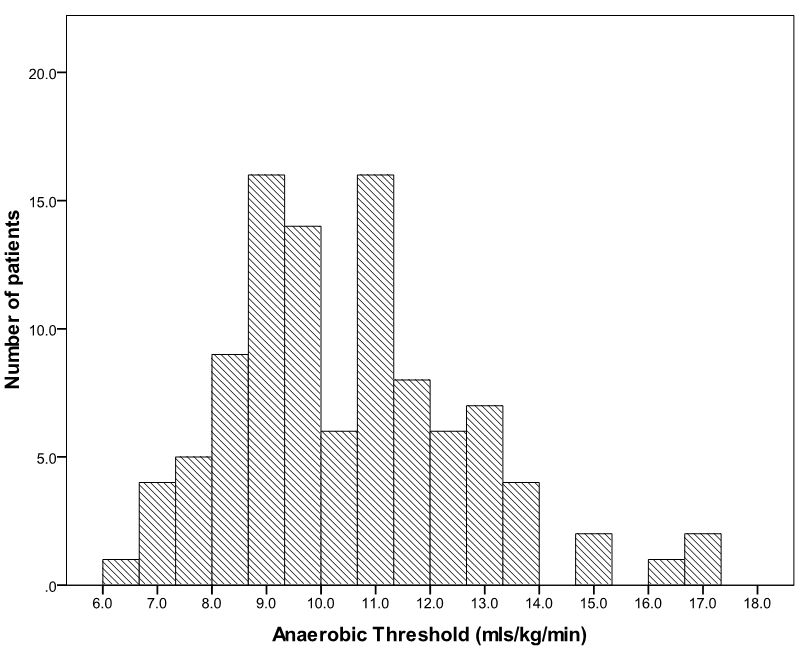
\includegraphics[width=0.8\linewidth]{Figures/cpet_outcomes_dist_of_AT}
	\caption{Distribution of VO$_2$AT across the study population.}
	\label{fig:cpet_outcomes_dist_of_AT}
\end{figure}

The relationship between VO$_2$AT and major postoperative adverse events including mortality is shown in Table \ref{table:cpet_outcomes_table2}. Patients with VO$_2$AT less than 10ml/kg/min had significantly greater incidence of postoperative pancreatic fistula (35.4\% vs.16\%, p=0.028) as well as major intra-abdominal abscesses (Clavien-Dindo Grade III - V, 22.4\% vs.7.8\%, p=0.042). While there was an association between low VO$_2$AT and grade of pancreatic fistula, this was not statistically significant (p=0.091). There was no association between low VO$_2$AT and cardiopulmonary complications or postoperative mortality. Major cardiopulmonary complications occurred more often in patients with major intra-abdominal adverse events including major intra-abdominal abscesses or Grade B and C pancreatic fistulae or haemorrhage than in patients who did not have these complications (5/31,16.1\% vs. 2/69,2.9\%, p=0.017). Postoperative mortality was not associated with VO$_2$AT (HR 0.77, 95\% CI 0.16-3.61, p 0.737) or the POSSUM Physiology Score (HR 0.39, 95\% CI 0.07-2.12, p 0.277). Postoperative mortality was associated with postoperative pancreatic fistula (n=5), post-pancreatectomy haemorrhage (n=3), major intra-abdominal sepsis (n=6) and major cardiorespiratory complications (n=4) with 6 patients requiring radiological or operative intervention.

%Table 2
\begin{table}[p]
	\centering
	\caption{The relationship between anaerobic threshold and complications in patients undergoing major pancreatic surgery.}
	\label{table:cpet_outcomes_table2}
	\renewcommand{\arraystretch}{1.2} %Increases space between rows
	\setlength{\tabcolsep}{12pt} %sets the space between columns

	
	\begin{tabular}{|C{1cm} l c c c c|}
		\hline
		\multicolumn{2}{|l}{Complications} &    & $\dot{V}_{O_2}$AT $\geq$10 & $\dot{V}_{O_2}$AT $<$ 10 &  \\
		 &                                 & n  & n                          & n                        & \textit{p} \\ \hline
		\multicolumn{6}{|l|}{Cardiac complications}                                                             \\
		 & Grade 0 - II                    & 99 & 51                         & 48                       & 0.308 \\
		 & Grade III - V                   & 1  & 0                          & 1                        &  \\
		\multicolumn{6}{|l|}{Respiratory complications}                                                         \\
		 & Grade 0 - II                    & 93 & 48                         & 45                       & 0.657 \\
		 & Grade III - V                   & 7  & 3                          & 4                        &  \\
		\multicolumn{6}{|l|}{Intra-abdominal abscess}                                                           \\
		 & Grade 0 - II                    & 85 & 47                         & 38                       & 0.042 \\
		 & Grade III - V                   & 15 & 4                          & 11                       &  \\
		\multicolumn{6}{|l|}{Pancreatic Fistula (Total/Sub-total pancreatectomies excluded)}                    \\
		 & No                              & 73 & 42                         & 31                       & 0.028 \\
		 & Yes                             & 25 & 8                          & 17                       &  \\
		\multicolumn{6}{|l|}{Pancreatic Fistula (ISGPS Classification)}                                         \\
		 & No                              & 73 & 42                         & 31                       & 0.091 \\
		 & Grade A                         & 9  & 3                          & 6                        &  \\
		 & Grade B                         & 8  & 1                          & 7                        &  \\
		 & Grade C                         & 8  & 4                          & 4                        &  \\
		\multicolumn{6}{|l|}{Post-Pancreatectomy Haemorrhage (ISGPS Classification)}                            \\
		 & No                              & 84 & 41                         & 43                       & 0.207 \\
		 & Grade A                         & 4  & 2                          & 2                        &  \\
		 & Grade B                         & 4  & 2                          & 2                        &  \\
		 & Grade C                         & 8  & 6                          & 2                        &  \\
		\multicolumn{6}{|l|}{Admissions to critical care}                                                       \\
		 & 1                               & 74 & 38                         & 36                       & 0.906 \\
		 & $>$1                            & 26 & 13                         & 13                       &  \\
		\multicolumn{6}{|l|}{Reoperation}                                                                       \\
		 & No                              & 89 & 47                         & 42                       & 0.306 \\
		 & Yes                             & 11 & 4                          & 7                        &  \\
		\multicolumn{6}{|l|}{Operative mortality}                                                               \\
		 & No                              & 93 & 47                         & 46                       & 0.737 \\
		 & Yes                             & 7  & 4                          & 3                        &  \\ \hline
		 \multicolumn{6}{l}{\textit{p} - Chi-square test}                                                               \\
	\end{tabular}
\end{table}

The median length of postoperative stay was 17 days (IQR 13 - 26). The median cumulative length of stay in critical care was 7 days (IQR 6 - 12). Twenty-six patients were admitted to critical care more than once. The relationship between preoperative clinico-pathological characteristics and length of postoperative stay in patients who were discharged from hospital (n=93) is shown in Table \ref{table:cpet_outcomes_table3}. On univariate analysis, age over 65 years (p=0.072) and low VO$_2$AT (p=0.010) were associated with prolonged postoperative stay. On multivariate Cox proportional hazards regression analysis, VO$_2$AT less than 10ml/kg/min (hazard ratio 1.74, 95\% confidence intervals 1.14-2.65, p=0.010) was the only significant factor associated with prolonged postoperative stay. A Kaplan-Meier plot for the probability of remaining in hospital over time for patients with low and normal VO$_2$ATs is shown in Figure \ref{fig:cpet_outcomes_km_at_los}. Patients with a low VO$_2$AT stayed a median 6 days longer in hospital (14 versus 20 days, Mann-Whitney Test p=0.001). There was no significant association between any of the preoperative factors including VO$_2$AT and length of critical care stay or number of critical care admissions.

% Table 3
\begin{table}[p]
	\centering
	\caption{The relationship between clinico-pathological characteristics and postoperative stay in patients (excluding operative mortality) undergoing major pancreatic surgery (n=93): Cox regression analysis}
	\label{table:cpet_outcomes_table3}
	\renewcommand{\arraystretch}{1.2} %Increases space between rows
	\setlength{\tabcolsep}{9pt} %sets the space between columns

	\begin{tabular}{|C{1cm} l c c c c c c c|}
		\hline
		\multicolumn{2}{|l}{Variable} & n  & HR   & 95\% CI   & P     & HR   & 95\% CI   & p     \\ \hline
		\multicolumn{9}{|l|}{Age (years)}                                                       \\
		 & $\leq$ 65                 & 44 &      &           &       &      &           &  \\
		 & $>$ 65                    & 49 & 1.47 & 0.97-2.24 & 0.072 & 1.48 & 0.97-2.25 & 0.068 \\
		\multicolumn{9}{|l|}{Sex}                                                               \\
		 & Male                      & 56 &      &           &       &      &           &  \\
		 & Female                    & 37 & 1.32 & 0.86-2.03 & 0.199 &      &           &  \\
		\multicolumn{9}{|l|}{BMI (kg/sq.m)}                                                     \\
		 & $\leq$ 25                 & 42 &      &           &       &      &           &  \\
		 & $>$ 25                    & 51 & 0.87 & 0.58-1.32 & 0.512 &      &           &  \\
		\multicolumn{9}{|l|}{Smoking}                                                           \\
		 & No                        & 56 &      &           &       &      &           &  \\
		 & Yes                       & 37 & 1.26 & 0.82-1.94 & 0.294 &      &           &  \\
		\multicolumn{9}{|l|}{POSSUM Physiology Score}                                           \\
		 & $\leq$ 14                 & 45 &      &           &       &      &           &  \\
		 & $>$ 14                    & 48 & 1.28 & 0.85-1.95 & 0.24  &      &           &  \\
		\multicolumn{9}{|l|}{Preoperative Biliary Drainage}                                     \\
		 & No                        & 53 &      &           &       &      &           &  \\
		 & Yes                       & 40 & 1.08 & 0.71-1.65 & 0.724 &      &           &  \\
		\multicolumn{9}{|l|}{Serum Bilirubin (micromol/L)}                                      \\
		 & $\leq$  35                & 54 &      &           &       &      &           &  \\
		 & $>$  35                   & 39 & 1.26 & 0.83-1.92 & 0.277 &      &           &  \\
		\multicolumn{9}{|l|}{mGPS}                                                              \\
		 & 0                         & 59 &      &           &       &      &           &  \\
		 & 1                         & 5  & 1.22 & 0.78-1.92 & 0.387 &      &           &  \\
		 & 2                         & 29 & 1.87 & 0.71-4.88 & 0.204 &      &           &  \\
		\multicolumn{9}{|l|}{Haemoglobin (g/dl)}                                                \\
		 & $\geq$ 12                 & 57 &      &           &       &      &           &  \\
		 & $<$ 12                    & 36 & 1.19 & 0.78-1.81 & 0.422 &      &           &  \\
		\multicolumn{9}{|l|}{Anaerobic Threshold  (ml/kg/min)}                                  \\
		 & $\geq$ 10                 & 47 &      &           &       &      &           &  \\
		 & $<$ 10                    & 46 & 1.74 & 1.14-2.64 & 0.01  & 1.74 & 1.14-2.65 & 0.01  \\
		\multicolumn{9}{|l|}{Anaerobic Threshold (ml/kg/min)}                                   \\
		 & $\geq$ 11                 & 33 &      &           &       &      &           &  \\
		 & $<$ 11                    & 60 & 1.44 & 0.94-2.22 & 0.097 &      &           & 0.395 \\ \hline
	\end{tabular}
\end{table}

% Figure 2
\begin{figure}[h]
\centering
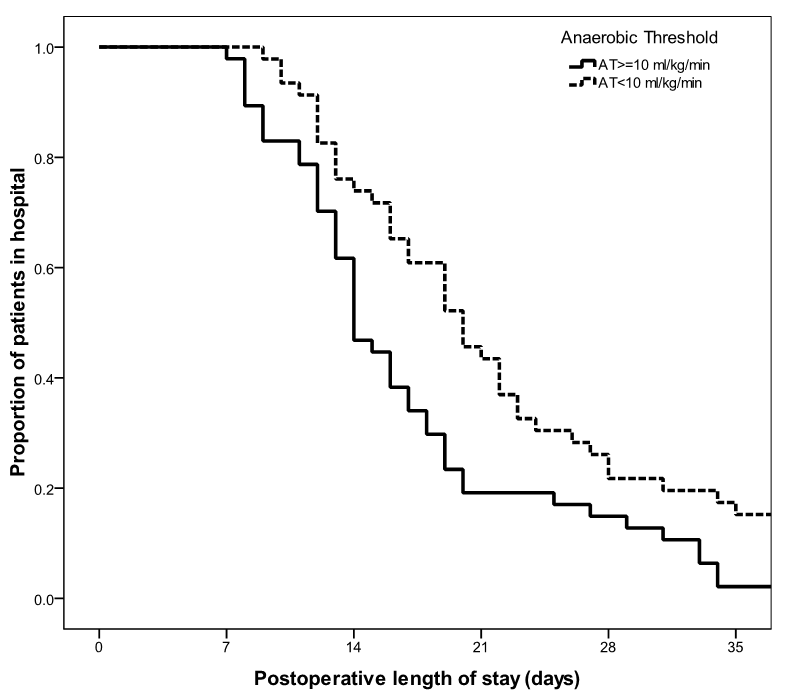
\includegraphics[width=0.8\linewidth]{Figures/cpet_outcomes_km_at_los}
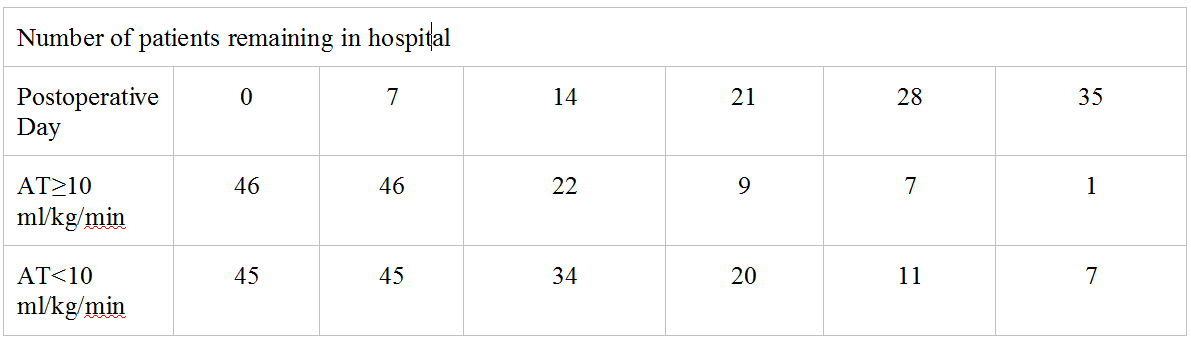
\includegraphics[width=1\linewidth]{Figures/cpet_outcomes_km_at_los_table} %Table below Kaplan Meier curve
\caption{Kaplan-Meier Plot of postoperative length of stay in patients with VO$_2$AT $>=$ 10ml/kg/min versus $<$ 10ml/kg/min.}
\label{fig:cpet_outcomes_km_at_los}
\end{figure}

The relationship between clinico-pathological patient factors and receipt of adjuvant therapy is shown in Table \ref{table:cpet_outcomes_table4}. Fifty-five patients were included in the analysis. Patients were excluded if chemotherapy was not indicated (n=28), in the event of operative mortality (n=7), if chemotherapy was offered but declined by the patient (n=4), or where they had not been seen by an oncologist yet (n=6). On binary logistic regression analysis, VO$_2$AT less than 10ml/kg/min was the only preoperative factor that was associated with with non-receipt of adjuvant therapy (HR 6.30, 95\% CI 1.25-31.75, p=0.026). 

%Table 4
\begin{table}[p]
	\caption{The relationship between clinico-pathological characteristics and receipt of adjuvant therapy in patients undergoing major pancreatic surgery (n = 55) - Binary logistic regression}
	\label{table:cpet_outcomes_table4}
	\centering
	\renewcommand{\arraystretch}{1.2} %Increases space between rows
	\setlength{\tabcolsep}{14pt} %sets the space between columns
	\begin{tabular}{|C{1cm} l c c c c|}
		\hline
		\multicolumn{2}{|l}{Variable} & n = 55 & HR   & 95\% CI    & \textit{p}    \\ \hline
		\multicolumn{6}{|l|}{Age (years)}                                  \\
		 & $\leq$ 65                  & 25     &      &            &  \\
		 & $>$ 65                     & 30     & 2.63 & 0.71-9.74  & 0.149 \\
		\multicolumn{6}{|l|}{Sex}                                          \\
		 & Male                       & 31     &      &            &  \\
		 & Female                     & 24     & 2.08 & 0.61-7.13  & 0.242 \\
		\multicolumn{6}{|l|}{BMI (kg/m$^2$)}                               \\
		 & $\leq$ 25                  & 25     &      &            &  \\
		 & $>$ 25                     & 30     & 0.78 & 0.23-2.64  & 0.693 \\
		\multicolumn{6}{|l|}{Smoking}                                      \\
		 & No                         & 35     &      &            &  \\
		 & Yes                        & 20     & 0.96 & 0.27-3.41  & 0.953 \\
		\multicolumn{6}{|l|}{POSSUM Physiology Score}                      \\
		 & $\leq$ 14                  & 25     &      &            &  \\
		 & $>$ 14                     & 30     & 1.63 & 0.46-5.73  & 0.447 \\
		\multicolumn{6}{|l|}{Preoperative Biliary Drainage}                \\
		 & No                         & 27     &      &            &  \\
		 & Yes                        & 28     & 0.95 & 0.28-3.21  & 0.937 \\
		\multicolumn{6}{|l|}{Serum Bilirubin ($\mu$mol/L)}                 \\
		 & $\leq$  35                 & 27     &      &            &  \\
		 & $>$  35                    & 28     & 2.08 & 0.60-7.30  & 0.251 \\
		\multicolumn{6}{|l|}{modified Glasgow Prognostic Score (mGPS)}     \\
		 & 0                          & 32     &      &            &  \\
		 & 1                          & 2      & 0    & 0          &  \\
		 & 2                          & 21     & 1.2  & 0.35-4.15  & 0.773 \\
		\multicolumn{6}{|l|}{Haemoglobin (g/dl)}                           \\
		 & $\geq$ 12                  & 31     &      &            &  \\
		 & $<$ 12                     & 24     & 0.96 & 0.28-3.26  & 0.946 \\
		\multicolumn{6}{|l|}{Anaerobic Threshold  (ml/kg/min)}             \\
		 & $\geq$ 10                  & 23     &      &            &  \\
		 & $<$ 10                     & 32     & 6.3  & 1.25-31.75 & 0.026 \\
		\multicolumn{6}{|l|}{Anaerobic Threshold  (ml/kg/min)}             \\
		 & $\geq$ 11                  & 16     &      &            &  \\
		 & $<$ 11                     & 39     & 3.11 & 0.61-15.88 & 0.172 \\ \hline
	\end{tabular}
	 %\todo{These AT numbers dont make sense. Why are there more patients with low AT? Check this.}
	 %These numbers are correct. Should I use simple chi-square test instead?
\end{table}

\clearpage

\section{Discussion}
The results of the present study show that a low VO$_2$AT is associated with prolonged postoperative stay in hospital, postoperative pancreatic fistula and intra-abdominal abscesses in patients undergoing major resections for pancreatic head lesions. The results of this study also show that patients with low VO$_2$AT are less likely to receive adjuvant therapy. 

Therefore, it would appear that objective measurement of patient physiological fitness using cardiopulmonary exercise testing is superior to conventional measures of patient fitness including the POSSUM Physiology Score or the modified Glasgow Prognostic Score and may have a role in predicting short-term outcome which in turn affects the overall management of these patients including receipt of adjuvant therapy.

Patients with a low VO$_2$AT stayed longer in hospital after their operation. While length of stay in hospital is influenced by multiple factors including postoperative complications, it would appear that patients with a low VO$_2$AT take longer to recover from the physiological stress placed by major pancreatic surgery and its sequelae.

The incidence of pancreatic fistula was greater in patients with a low VO$_2$AT. This association needs further evaluation taking into consideration other well-recognised risk factors for pancreatic fistula such as pancreatic texture, pancreatic duct size and intra-operative blood loss.\parencite{braga_prognostic_2011, pratt_possum_2008, winter_1423_2006} It is possible that local or operative factors may be compounded by poor oxygen delivery and organ perfusion as measured by cardiopulmonary exercise testing. There was a non-significant trend towards clinically relevant pancreatic fistulae (ISGPS Grades B and C) as well as a significant association with major intra-abdominal abscesses (Clavien-Dindo Grades 3-5 i.e., requiring intervention, associated with organ dysfunction requiring intensive care or resulting in mortality). This would suggest that complications in patients with low VO$_2$AT are more likely to be severe than in patients with normal VO$_2$AT. However, there was no difference in mortality between patients with normal or low VO$_2$AT, indicating that multiple factors including preoperative patient fitness, local and operative factors, systemic inflammatory response, number of complications as well as perioperative critical care all play a role.

The results of this study also show that patients with a low VO$_2$AT were less likely to receive adjuvant therapy. Adjuvant therapy in patients undergoing pancreatic resections for cancer has been shown in multiple randomised trials to improve survival significantly.\parencite{neoptolemos_randomized_2004, neoptolemos_adjuvant_2009}
While postoperative mortality after pancreatic surgery has steadily improved over the years with major improvements in the quality of surgical and critical care over the past decade\parencite{winter_1423_2006} even in elderly patients\parencite{makary_pancreaticoduodenectomy_2006}, postoperative morbidity remains high.\parencite{mann_review_2010} The results of this study show that poor preoperative fitnees is not only associated with a protracted protracted postoperative course with complications but also with non-receipt of adjuvant therapy.

In the present study, VO$_2$AT was less than 10ml/kg/min in 49\% of patients and less than 11 ml/kg/min in 64\% of patients. The proportion of patients with VO$_2$AT less than 11 ml/kg/min in this study was much greater than reported in studies involving patients undergoing oesophageal surgery (16\%),\parencite{forshaw_is_2008} liver transplantation (39\%)\parencite{epstein_aerobic_2004} or other major abdominal surgery (29\%)\parencite{older_preoperative_1993} and may indicate the poor preoperative fitness levels of patients undergoing major pancreatic surgery at our unit. While several studies have shown that low VO$_2$AT and/or low VO$_2$peak are associated with postoperative complications or prolonged hospital stay following major abdominal surgery as well as non-abdominal surgery,\parencite{older_preoperative_1993, epstein_aerobic_2004, mccullough_cardiorespiratory_2006, nagamatsu_preoperative_2001, older_cardiopulmonary_1999, older_clinical_2004} others have disputed this.\parencite{forshaw_is_2008, clayton_cardiopulmonary_2011, hightower_pilot_2010} Older and co-workers reported in 1993 that low VO$_2$AT less than 11ml/kg/min was associated with a significantly higher risk of postoperative mortality from cardiovascular causes in a series of 187 elderly patients undergoing major abdominal surgery.\parencite{older_preoperative_1993}

However, Snowden and co-workers\parencite{snowden_submaximal_2010} reported that patients with an VO$_2$AT less than 10.1 ml/kg/min had significantly greater cardiopulmonary complications as well as non-cardiopulmonary and infectious complications while Forshaw and co-workers\parencite{forshaw_is_2008} reported that using a cut-off of 11 ml/kg/min for the VO$_2$AT did not predict postoperative adverse events less after oesophagectomy. The lack of association between low VO$_2$AT and cardiopulmonary complications in this study may have been due to two reasons. Major cardiopulmonary complications occurred more often in association with major intra-abdominal adverse events which are determined largely by pancreatic morphology and local anatomy.\parencite{braga_prognostic_2011} Moreover, the stringent fitness criteria for undergoing pancreaticoduodenectomy may have excluded patients with known co-morbid cardiorespiratory diseases such as severe chronic obstructive pulmonary disease or cardiac failure.

The results of this study are consistent with the results of the study by Ausania and co-workers\parencite{ausania_effects_2012} who reported increased incidence of pancreatic fistula and prolonged postoperative stay in patients with VO$_2$AT less than 10.1 ml/kg/min. However, this study did not report the association between VO$_2$AT and receipt of adjuvant therapy.

The physiological demands placed on a patient undergoing major pancreatic surgery are significant, both during and after the operation. It is not entirely surprising therefore, that conventional parameters of patient fitness like the POSSUM Physiology Score or the modified Glasgow Prognostic Score are limited in their ability to distinguish patients based on their performance under physiological stress. Cardiopulmonary exercise testing overcomes this disadvantage by replicating some of the physiological burden major pancreatic surgery places on the functional capacity of the patient's cardiovascular and respiratory systems.

This functional capacity of patients to withstand the physiological burden of major surgery can be improved by the process of ‘prehabilitation’.\parencite{topp_effect_2002} It has been suggested that prehabilitation not only improves aerobic capacity\parencite{jones_effects_2007} but may also improve postoperative recovery.\parencite{mayo_impact_2011, pehlivan_effects_2011} The results of this study show that impaired aerobic capacity is associated with postoperative adverse events. Therefore, it would appear that prehabilitation using interventions such as exercise and nutrition, by improving physiological fitness, may have a role in improving postoperative outcomes after major pancreatic surgery and may improve the proportion of patients receiving adjuvant therapy.

Further work needs to be carried out to study the value of cardiopulmonary exercise testing in predicting postoperative complications in conjunction with previously established factors such as pancreatic morphology and operative factors before it can be used on its own to select or exclude patients for pancreaticoduodenectomy. Cardiopulmonary exercise testing would play an important role not only in identifying patients who will benefit from prehabilitation, but also in the objective measurement of the effects of such interventions on aerobic capacity as well as in identifying high risk patients who may not be able to complete oncological treatment. Prehabilitation and optimised perioperative care may allow a greater proportion of high risk patients to progress to oncological treatment after surgery.